\section{Introduction}
\label{sec:introduction}
Uncertain and multivariate data visualizations were viewed as major challenges during a visualization seminar at Daghstuhl in 2011, leading to a book~\cite{hansen2014scientific} providing an overview of the domain. 
%
Although scientific data extracted from computational simulations are often both uncertain and multivariate in nature, efforts to develop visualization techniques for these data types have been pursued independently due to the challenges involved.
%
In this paper, we build upon a recent advancement in multivariate data visualization and extend an existing univariate uncertain data visualization technique to enable uncertain multivariate data visualization.

Recently, Jankowai and Hotz~\cite{jankowai2020feature} proposed a technique for surface-based visualization of complex features in multivariate data called \textit{feature level-sets}. 
%
Feature level-sets are the generalization of isosurfaces to multivariate data.
%
They are surfaces in the spatial domain initialized by the distance field generated for a \textit{trait} defined in attribute space.
%
The ``zero'' feature level-set corresponds to the feature in the spatial domain that matches the trait exactly.
%
In many cases, this feature is visualized using a small threshold distance to highlight the points in the domain that are closest to it. 
%
%Additional level-sets for larger distances show secondary feature structures. 
%

In this paper, we extend the existing approach of using \textit{confidence isosurfaces} to visualize uncertainty for univariate data~\cite{zehner2010visualization} to multivariate data via feature level-sets.
%
Specifically, we are interested in visualizing the uncertainty of the zero level-set.
%
We propose \textit{feature confidence level-sets}, the generalization of confidence isosurfaces to multivariate data.
%
%Our motivation is twofold.
%
To extract the zero level-set and the corresponding feature confidence level-sets, our approach utilizes distance fields computed in the spatial domain directly.
%
Our choice of distance metric enables selection of level-sets close to the feature guided by domain information~(extents and grid resolution).
%
While feature level-sets compute a distance field based on the distribution of a function in the domain, feature confidence level-sets additionally consider the uncertainty of the function, represented as a distribution at each grid point, in the domain.
%To compute a distance field irrespective of the metric, besides the distribution of a function in the domain as in feature level-sets, feature confidence level-sets consider the uncertainty, encoded as a distribution, at each grid point. 
%
%\fix{(I would suggest swapping the order of the first and second motivations. This is because the paragraph under second point really is a strong technical motivation. In the end, we may say our second motivation is that this area is unexplored to our best knowledge. One option is removing the sentence "our motivation is twofold", and in the end stating that the uncertainty vis of feature level-sets is unexplored area to the best of our knowledge.)}.
%
%presents the first uncertain multivariate spatial data visualization technique. 
%
%First, compared to feature level-sets alone, feature confidence level-sets could offer improved secondary feature structure visualization for uncertain multivariate data.
%
%In particular, Jankowai and Hotz have identified that a shortcoming of computing multiple feature level-sets using a single Euclidean distance is discernibility: points with equal distance to the feature cannot be distinguished in the final level-set rendering.
%%
%Further, we conjecture that as the Euclidean distance from the feature increases, the effectiveness and relevance of additional feature level-sets reduces for many applications.
%%
%In our approach, we compute distance fields based on the trait definition and additional fields based on the trait definition as well as a confidence percentage, and render level-sets extracted from these fields.
%%
%Rather than render multiple level-sets using $distance_{T}$, we only render $ZLS_{T}$ augmented with a feature confidence level-set, i.e., $FCLS_{T,C}$.
%
Further, to the best of our knowledge, we believe this work is the first to propose an uncertainty visualization technique for multivariate data based on feature level-sets. 
%
We demonstrate our technique using synthetic, real, and simulation uncertain multivariate data sets.
%, and qualitatively compare the results with using multiple level-sets initialized by $distance_{T}$. 

%In recent years, there has been increasing interest in the visualization of multivariate and uncertain data.
%%
%Uncertainty and multivariate data visualization were viewed as major challenges during a Visualization seminar at Daghstuhl in 2011, and led to a book~\cite{hansen2014scientific} providing an overview of the domain. 
%%
%Although most scientific data extracted from computational simulations is of, both, uncertain and multivariate nature, efforts to develop scientific visualization techniques for these data types has often been pursued independently due to the challenges involved.
%%
%
%Zehner et al.~\cite{zehner2010visualization} proposed an intuitive approach to visualize uncertainty for univariate data via the use of \textit{confidence isosurfaces} or glyphs~\cite{zehner2010visualization}.
%%
%In the case of multivariate data, individual confidence isosurfaces or gylphs for each variable, however, could lead to occlusion and has limited dimension scalability.
%%
%Recently, Jankowai and Hotz~\cite{jankowai2020feature} proposed a surface-based visualization technique for complex features in multivariate data called \textit{feature level-sets}. 
%%
%Feature-level sets are the generalization of isosurfaces to multivariate data.
%%
%They are surfaces $FLS_{T}$ in the spatial domain initialized by the distance field generated for a \textit{trait} $T$ defined in attribute space.
%%
%The ``zero'' feature level-set, $ZLS_{T}$, corresponds to the feature in the spatial domain that matches the trait exactly.
%%
%In many cases, the $ZLS_{T}$ is visualized using a small threshold distance to highlight the points in the domain that are closest to the feature in attribute space.
%%
%Additional level-sets for larger distances show secondary feature structures.
%%
%In this paper, to enable visualization of uncertain multivariate data we propose \textit{feature confidence level-sets}, the generalization of confidence isosurfaces to multivariate data via feature level-sets. 
%
%Besides offering the capability to visualize uncertain multivariate data, we believe feature confidence level-sets 
%%benefit from utilizing distribution information to produce level-sets 
%produce isosurfaces that improve secondary feature structure visualization.
%%
%In the original work, Jankowai and Hotz demonstrate feature level-sets using multiple level-sets initialized by a single distance field.
%%
%They identify that a shortcoming of computing multiple level-sets using a single Euclidean distance is discernibility, i.e., points with equal distance to the $ZLS_{T}$ cannot be distinguised in the final level-set rendering.
%%
%Further, we conjecture that as the Euclidean distance from the $ZLS_{T}$ increases, the effectiveness and relevance of additional feature level-sets reduces for many applications.
%%
%In our approach, we compute multiple distance fields: $distance_{T}$ based on the trait definition, and additional fields $distance_{T,C}$ based on the trait definition and a confidence interval percentage $C$. 
%%
%Rather than render multiple level-sets using $distance_{T}$, we only render $ZLS_{T}$ augmented with a feature confidence level-set, i.e., $FCLS_{T,C}$.
%%
%We demonstrate the technique using five uncertain multivariate data sets, and qualitatively compare the results with using multiple level-sets initialized by $distance_{T}$.
%
%%We organize the remainder of this paper as follows:
%%%
%%Section~\ref{sec:related} discusses work related to the presented technique. 
%%%
%%Section~\ref{sec:method} formally introduces feature confidence level-sets and specifies any limits in scope considered for this study.
%%%
%%In Section~\ref{sec:study}, we provide a short study overview, followed by our results in Section~\ref{sec:results}.
%%%
%%Finally, we discuss various aspects of possible future work and conclude in Section~\ref{sec:conclusion}


\section{Related Work}
\label{sec:related}
Feature confidence level-sets target scientific uncertain and multivariate spatial data.
%%
Although there have been efforts to visualize non-spatial uncertain multivariate data, they are limited for spatial data.
%%
For comprehensive overviews of these domains separately, we refer readers to state-of-the-art reports for uncertainty visualization~\cite{Bonneau2014} and multivariate spatial data visualization~\cite{he2019multivariate}.
%%
In this section, we restrict our discussion to works most relevant to this study.


In the recent past, there are two notable multivariate spatial data visualization efforts: fiber surfaces and feature level-sets.
%
Fiber surfaces proposed by Carr et al.~\cite{carr2015fiber} are the generalization of isosurfaces to bivariate data and involve modifying the Marching Cube's algorithm.
%
Klacansky et al.~\cite{klacansky2016fast} proposed a parallelized implementation to speedup generation of exact fiber surfaces.
%
Wu et al.~\cite{wu2016direct} perform accurate direct volume rendering of fiber surfaces using higher-order interpolation schemes.
%
More recently, fiber surfaces, have been extended to multivariate data by Blecha et al.~\cite{blecha2020fiber}.
%

Feature level-sets, as previously mentioned, are the generalization of isosurfaces to multivariate data and were proposed by Jankowai and Hotz~\cite{jankowai2020feature}.
%
In ~\cite{jankowai2020feature}, the authors identify multiple opportunities for future research including the definition of the distance metric, performance optimizations, trait specification interfaces, etc.
%
Nguyen et al.~\cite{nguyen2020visualization} proposed first smoothing of the distance field using Gaussian kernels before extracting level-sets to visualize coherent structures in Taylor-Couette turbulence flows.
%
Jankowai et al.~\cite{jankowai2020tensor} explored its application for tensor data. 
%
Further, the feature-level sets technique has been implemented for multivariate data visualization within the Inviwo visualization framework~\cite{jonsson2020inviwo}. 
%
In this paper, we extend and investigate the feature-level sets technique for uncertain multivariate data. 

There are several research works aiming to address uncertainty in scientific visualization.
%
However, faced with occlusion challenges these techniques have largely focused on univariate data~\cite{}.
%
In this work, we build upon the method by Zehner et al.~\cite{zehner2010visualization} to visualize uncertainty using confidence isosurfaces.
%
In addition to offering straightforward generalization to multivariate data, confidence isosurfaces are determined on the basis of a specific confidence interval percentage and thus, provides intuitive understanding of uncertainty by producing different shapes of isosurfaces due to uncertainty. 
%
In contrast, correctly identifying isovalues to render multiple level-sets often involves trial and error as well as spatial extents knowledge. 

%Feature level-sets are computed based on a trait specified in attribute space.
%%
%The trait is analogous to an isovalue for the univariate case, except that for a non-empty feature level-set the trait must exist in attribute space.
%%
%Traditionally, for a specific trait, first a binary volume is computed, followed by a Euclidean distance transform to generate a distance field, and lastly, isosurfacing of the distance field.
%%
%At a distance of zero (or a small threshold), the feature in the spatial domain as defined by the trait in attribute space can be extracted.
%%
%Additional level-sets can be extracted from the distance field to provide insight regarding the feature structure.
%%
%Figure~\ref{} illustrates the visualization pipeline for the generation of feature-level sets.
%
%%
%In this paper, we propose replacing the distance field level-sets with level-sets showing uncertainty. 
%%
%This approach in effect improves the performance of the visualization pipeline by eliminating the Euclidean distance transformation.
%%
%Instead, we compute binary volumes for the feature level-set and the feature confidence level-set. 
%%
%Zehner et al.~\cite{zehner2010visualization} proposed the use of isosurface envelopes to show confidence for the univariate case.
%%
%Using the same definition and extending it to the multivariate case, a feature confidence level-set indicates within which volume the feature will lie with a certain confidence.
%%
%We illustrate a notional example of a feature confidence level-set for bivariate data in Figure~\ref{}.


\section{Our Method}
\label{sec:method}
\setlength{\belowdisplayskip}{5pt} \setlength{\belowdisplayshortskip}{5pt}
\setlength{\abovedisplayskip}{5pt} \setlength{\abovedisplayshortskip}{5pt}

We begin with a description of our uncertain multivariate data and the corresponding attribute space, followed by a discussion of trait specification, choice of distance metric, generation of feature level-sets, and finally, generation of feature confidence level-sets.
%
Finally, Figure~\ref{fig:example} provides a notional example of the different steps involved to generate the level-sets and is referenced in Sections~\ref{sec:fls} and~\ref{sec:fcls}.
%

\vspace{-1mm}
\subsection{Uncertain Multivariate Data}
%
From~\cite{jankowai2020feature}, general multivariate data are a set of scalar, vector, or tensor fields $\{F_1,F_2,...,F_r\}$ in the domain $D \subset \mathbb{R}^{3}$, where $r\in\mathbb{N}$ and $r\geq2$.
%
%
%From~\cite{jankowai2020feature}, general multivariate data are a set of fields
%\begin{equation}
%\left\{F_{1},F_{2},...,F_{r}\right\}, r\in\mathbb{N}, F_{i}:D_{i} \to R_{i},
%\end{equation}
%where $D_{i} = D \subset \mathbb{R}^{3}$ for all $i$ and $R_{i}$ may be sets of scalar, vectors or tensors, and $r\geq2$.
%
Attribute space $\mathcal{A}$ is the combination of the field values and can further include derived quantities.
%
The dimensionality of $\mathcal{A}$ is the combined dimensionality of all selected field values or derived quantities.
%
Considering this definition of attribute space, multivariate data can be summarized as the mapping
\begin{equation}
f : D \to \mathcal{A} \subset R^{n},
\end{equation}
%
where $n$ is the number of dimensions used to form attribute space. 
%
%For our study, we used a maximum of $n = 3$. 
%

For uncertainty in each dimension $i$ of attribute space, we assumed the normal distribution of values at each grid point in $D$ and represented it using mean ${\mu}_{i}$ and standard deviation ${\sigma}_{i}$. 

\vspace{-2mm}
\subsection{Trait Specification}
Traits can be defined generally as artibrary geometries in attribute space $\mathcal{A}$ whose equivalent counterparts in the spatial domain $D$ are identified as features, i.e., $T\subset\mathcal{A}$.
%
A trait can be of any dimension and structure, including points, intervals, lines, and volumes.
%
%The specification of complex traits in a high-dimensional attribute space is a non-trivial task.
%
For simplicity, we assume a limited definition of a trait $T$ by considering intervals for each dimension $i$ of attribute space $\mathcal{A}$
%
\begin{equation}	
T = \forall{i}\;[L_{i}, U_{i}], \;\;L_{i} \leqslant U_{i}, 
\end{equation}
where $L_{i}$ is the lower bound, and $U_{i}$ is the upper bound of the interval for each dimension.
%
As an example, in a visualization of $\mathcal{A}$ for $n = 2$ using a scatterplot, a trait by our definition would be a rectangular selection.

\vspace{-1mm}
\subsection{Distance Metric}
%
%We assume a non-empty feature for our selection of trait $T$.

The feature and feature confidence level-sets are extracted from distance fields.
%
Our objective is to visualize the feature and feature confidence level-sets via the corresponding zero level-sets~(see Sections~\ref{sec:fls} and~\ref{sec:fcls}, respectively). 
%
To achieve this, we computed distance fields using the Euclidean distance transformation~(EDT) algorithm by Saito et al.~\cite{saito1994new} in the spatial domain directly.
%
The field derived from the EDT algorithm is computed for each grid point in the spatial domain and encodes the distance from a feature.
%
A distance field computed in the spatial domain allows a domain information-guided selection of small threshold distances, whereas distance fields derived from attribute space can be harder to interpret due to dynamic ranges among attributes.
%
In ~\cite{jankowai2020feature}, the distance field is computed in attribute space to address empty features.
%
In the event that a trait $T$ results in an empty feature, our choice of distance metric would result in a constant distance field.
%

\vspace{-1mm}
\subsection{Feature Level-Sets}
\label{sec:fls}
In general, a feature is defined as the pre-image of the trait $T$ in the spatial domain
\begin{equation}
f^{-1}(T) = \left\{ x \in D |\; f(x) \in T \right\}
\end{equation}
%
For our limited definition of a trait $T$ and ${\mu}_{i}$ field of each dimension, a feature is defined as 
\begin{equation}
f^{-1}(T) = \left\{ x \in D |\; \forall i\;{\mu}_{i}(x) \cap [L_{i}, U_{i}] \neq \emptyset\right\}
\end{equation}

To visualize the feature and its secondary structures, we performed three steps:
%
First, for trait $T$, we computed a binary volume $bvolume_{T}$~(Figure~\ref{fig:bvolumeT}) to represent the absence or existence of the feature at a specific grid point
%
\begin{equation}
  bvolume_{T}(x) = \left \{
  \begin{aligned}
    &0, && \text{if}\; \forall i\; {\mu}_{i}(x) \cap [L_{i}, U_{i}] \neq \emptyset \\
    &1, && \text{otherwise}
  \end{aligned} \right.
\end{equation}
%
Second, we performed EDT using $bvolume_{T}$ as input to produce a distance field $distance_{T}$~(Figure~\ref{fig:distanceT}). 
%
%We used an algorithm proposed by Saito \textit{et al.}~\cite{saito1994new} to perform EDT.
%
As a final step, we computed feature level-set $FLS_{T,K}$ as the level-set of level $K$ of the distance field
%
\begin{equation} 
distance_{T}^{-1}(K) = \left\{ x \in D\; |\; distance_{T}(x) = K\right\}
\end{equation}
%
$K$ is the spatial distance from $\forall i\; \mu_{i}(x) \cap [L_{i}, U_{i}] \neq \emptyset$.
%
For $K = \epsilon$, i.e., a small threshold value near zero, we refer to $FLS_{T,\epsilon}$ as $ZLS_{T}$~(Figure~\ref{fig:zlsT}).
%\fix{Figure~\ref{fig:example} top row illustrates the different steps to generate $FLS_{T,\epsilon}$ or $ZLS_{T}$.}
%
%As the value of $K$ increases, we believe \fix{(instead of saying "we believe", should we refer to ~\cite{jankowai2020feature}, as we did in the Introduction last paragraph?)} its relevance reduces given discernibility concerns and greater distance from the feature in the spatial domain.
%

\begin{figure}[!b]
\vspace{-5mm}
\centering
\begin{subfigure}{0.243\linewidth}
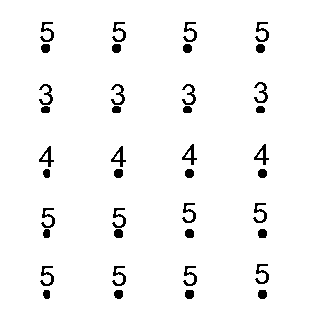
\includegraphics[width=\linewidth]{Images/mu.pdf}
\vspace{-5mm}
\caption{${\mu}$}
\label{fig:mu}
\end{subfigure}
\begin{subfigure}{0.243\linewidth}
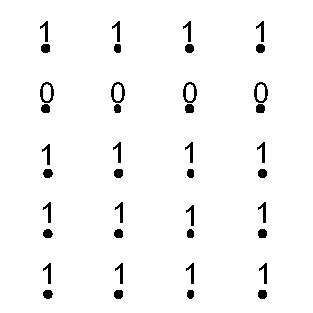
\includegraphics[width=\linewidth]{Images/bvolumeT.pdf}
\vspace{-5mm}
\caption{$bvolume_{T}$}
\label{fig:bvolumeT}
\end{subfigure}
\begin{subfigure}{0.243\linewidth}
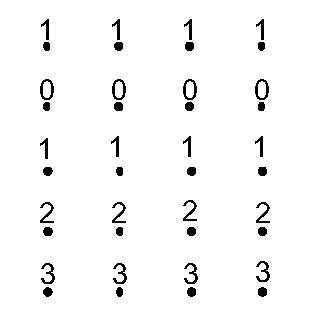
\includegraphics[width=\linewidth]{Images/distanceT.pdf}
\vspace{-5mm}
\caption{$distance_{T}$}
\label{fig:distanceT}
\end{subfigure}
\begin{subfigure}{0.243\linewidth}
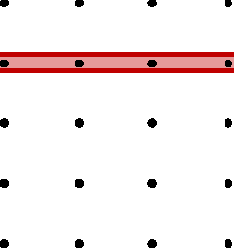
\includegraphics[width=\linewidth]{Images/zlsT.pdf}
\vspace{-5mm}
\caption{$ZLS_{T}$}
\label{fig:zlsT}
\end{subfigure}
\begin{subfigure}{0.243\linewidth}
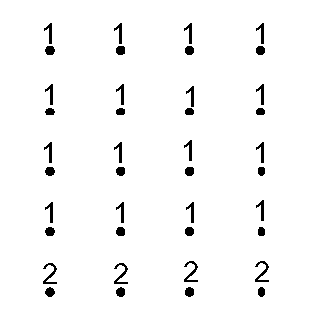
\includegraphics[width=\linewidth]{Images/sigma.pdf}
\vspace{-5mm}
\caption{${\sigma}$}
\label{fig:sigma}
\end{subfigure}
\begin{subfigure}{0.243\linewidth}
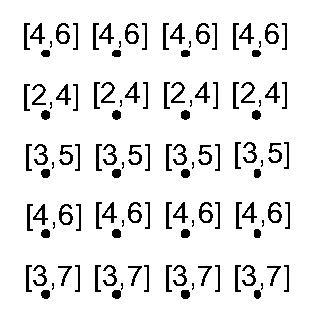
\includegraphics[width=\linewidth]{Images/boundsC.pdf}
\vspace{-5mm}
\caption{$bounds_{C}$}
\label{fig:boundsC}
\end{subfigure}
\begin{subfigure}{0.243\linewidth}
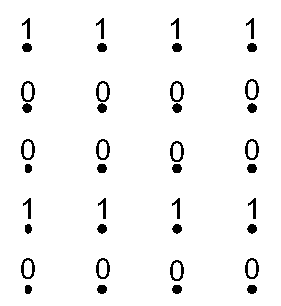
\includegraphics[width=\linewidth]{Images/bvolumeTC.pdf}
\vspace{-5mm}
\caption{$bvolume_{T,C}$}
\label{fig:bvolumeTC}
\end{subfigure}
\begin{subfigure}{0.243\linewidth}
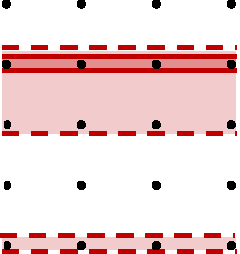
\includegraphics[width=\linewidth]{Images/zlsT_fclsTC.pdf}
\vspace{-5mm}
\caption{{\scriptsize $ZLS_{T}$+$FCLS_{T,C}$}}
\label{fig:fclsTC}
\end{subfigure}
\caption{A notional example showing the steps involved in generating the ``zero'' feature level-set $ZLS_{T}$~(top row) and feature confidence level-set $FCLS_{T,C}$~(bottom row) for an uncertain univariate field represented using ${\mu}$~(a) and ${\sigma}$~(e).
%
For this example, we use trait $T=[2.5, 3.5]$ and confidence $C=68\%$, i.e., $Z=1$.
%
$FCLS_{T,C}$ is computed using the $distance_{T,C}$ (not shown) field.
%
Assuming a unit distance between adjacent grid points,
%
$distance_{T,C}$ would be computed using $bvolume_{T,C}$~(g) as input and would appear equivalent for this example.
%$bvolume_{T,C}$~(g) and $distance_{T,C}$ (not shown) would appear equivalent for this example.
}
\label{fig:example}
\vspace{-5mm}
\end{figure}

\begin{figure*}[!h]
\begin{subfigure}{0.195\linewidth}
\centering
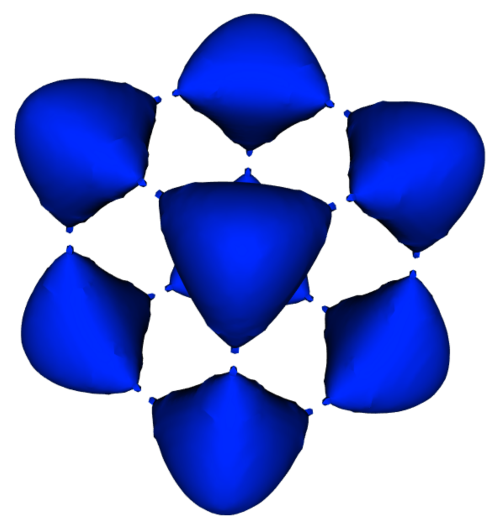
\includegraphics[width=0.8\linewidth]{Images/Tangle/gt.pdf}
\vspace{-2mm}
\caption{Ground truth, $isoval=62$}
\label{fig:tangle_gt}
\end{subfigure}
\begin{subfigure}{0.195\linewidth}
\centering
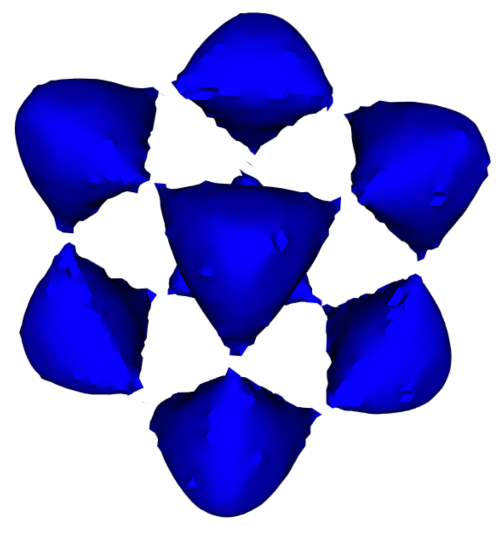
\includegraphics[width=0.8\linewidth]{Images/Tangle/zls.pdf}
\vspace{-2mm}
\caption{$ZLS_{T}$}
\label{fig:tangle_zls}
\end{subfigure}
\begin{subfigure}{0.195\linewidth}
\centering
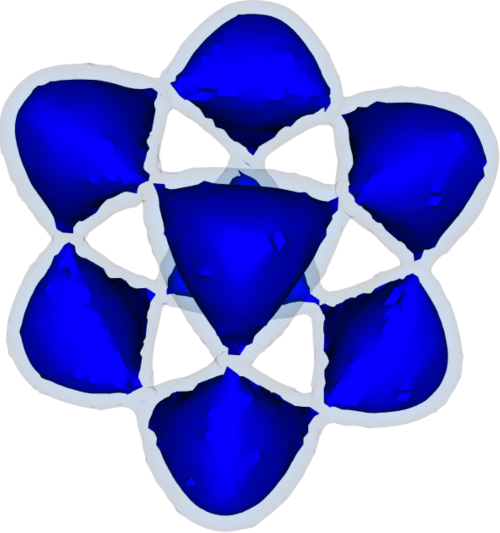
\includegraphics[width=0.8\linewidth]{Images/Tangle/fls.pdf}
\vspace{-2mm}
\caption{$ZLS_{T}$ + $FLS_{T,2}$}
\label{fig:tangle_fls}
\end{subfigure}
\begin{subfigure}{0.195\linewidth}
\centering
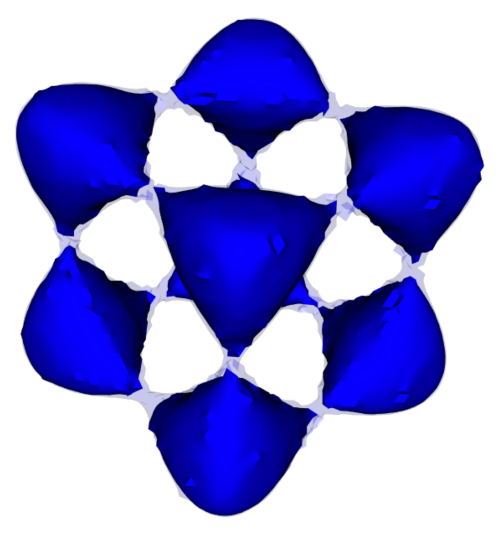
\includegraphics[width=0.8\linewidth]{Images/Tangle/fcls_68.pdf}
\vspace{-2mm}
\caption{$ZLS_{T}$ + $FCLS_{T,68\%}$}
\label{fig:tangle_fcls_68}
\end{subfigure}
\begin{subfigure}{0.195\linewidth}
\centering
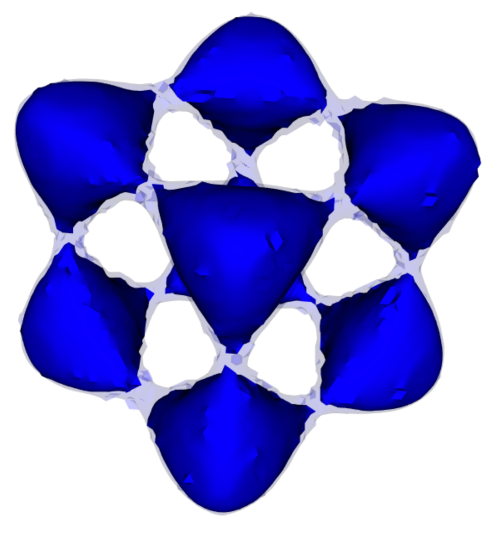
\includegraphics[width=0.8\linewidth]{Images/Tangle/fcls_95.pdf}
\vspace{-2mm}
\caption{$ZLS_{T}$ + $FCLS_{T,95\%}$}
\label{fig:tangle_fcls_95}
\end{subfigure}
\vspace{-2mm}
\caption{Visualization of sensitivity of the tangle function near values that form links between the multiple blobs. We use $T=[0,62]$.}
\vspace{-2mm}
\label{fig:tangle}
\end{figure*}

\begin{figure*}[!h]
\begin{subfigure}{0.20\linewidth}
\centering
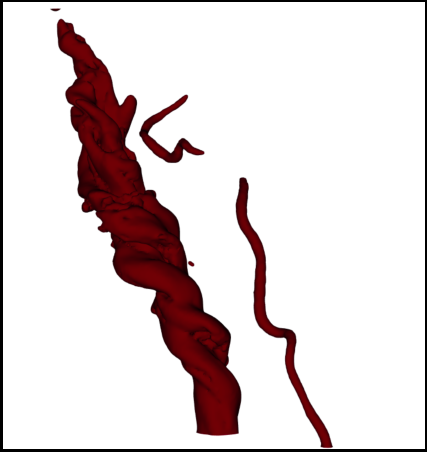
\includegraphics[width=0.9\linewidth]{Images/Tornado/zls.pdf}
\vspace{-1mm}
\caption{$ZLS_{T}$}
\label{fig:tornado_zls}
\end{subfigure}
\begin{subfigure}{0.20\linewidth}
\centering
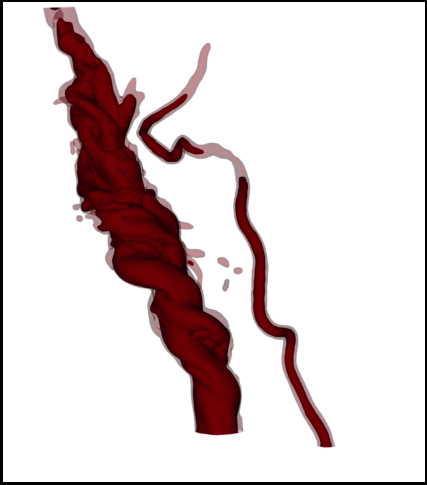
\includegraphics[width=0.9\linewidth]{Images/Tornado/fcls_50.pdf}
\vspace{-1mm}
\caption{+ $FCLS_{T,50\%}$}
\label{fig:tornado_fls}
\end{subfigure}
\begin{subfigure}{0.20\linewidth}
\centering
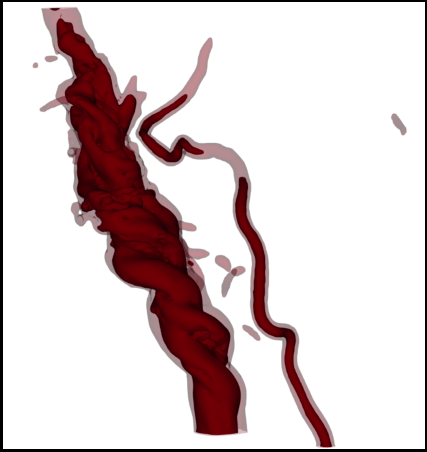
\includegraphics[width=0.9\linewidth]{Images/Tornado/fcls_68.pdf}
\vspace{-1mm}
\caption{+ $FCLS_{T,68\%}$}
\label{fig:tornado_fls}
\end{subfigure}
\begin{subfigure}{0.20\linewidth}
\centering
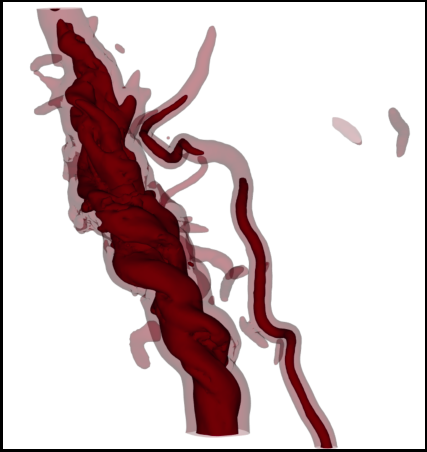
\includegraphics[width=0.9\linewidth]{Images/Tornado/fcls_95.pdf}
\vspace{-1mm}
\caption{+ $FCLS_{T,95\%}$}
\label{fig:tornado_fcls}
\end{subfigure}
\hfill
\begin{subfigure}{0.17\linewidth}
\centering
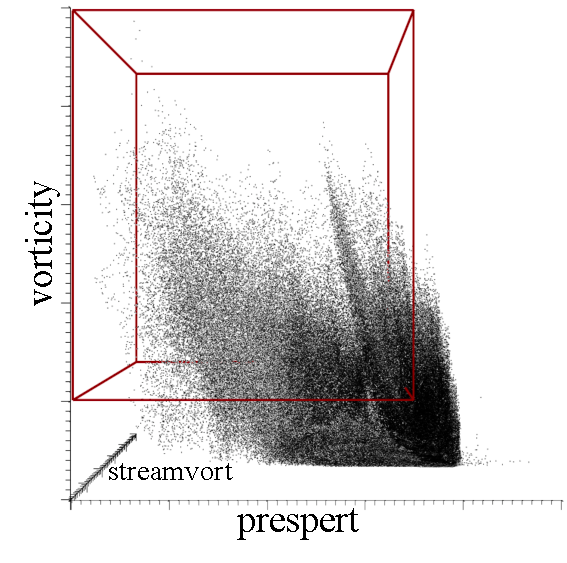
\includegraphics[width=\linewidth]{Images/Tornado/scatterplot3d.pdf}
\vspace{-4mm}
\caption{3D scatterplot of $\mathcal{A}$ and $T$ (red cuboid).} 
\label{fig:tornado_scatterplot}
\end{subfigure}
%\vspace{-2mm}
\caption{Visualization of EF-5 tornado vortices using vorticity, prespert and streamvort attributes. As in Figure~\ref{fig:tangle}, $FCLS_{T,C}$ formed wider envelopes as $C$ increased. Importantly, $FCLS_{T,C}$ visualized vortical structures of interest in the vicinity of the primary tornado vortex.}
%\vspace{-1mm}
\label{fig:tornado}
\end{figure*}


\vspace{-1mm}
\subsection{Feature Confidence Level-Sets}
\label{sec:fcls}
%
Uncertainty in multivariate data can result in different shapes of $ZLS_{T}$.
%
To assess the uncertainty, we visualized within which envelope the $ZLS_{T}$ will lie for a certain confidence interval $C$.
%
Similar to the steps we used to compute $ZLS_{T}$, to extract feature confidence level-sets $FCLS_{T,C}$, we first identified all the grid points that satisfy the trait $T$ for confidence interval $C$.
%
To achieve this, we used the method by Zehner et al.~\cite{zehner2010visualization}. 
%
We used the $Z$-score, or the number of standard deviations from the mean a value would be, for a given confidence interval $C$, and then, for each dimension $i$, calculated $bounds_{i,C}$~(Figure~\ref{fig:boundsC})
%\fix{(should we replace variable C with variable Z, e.g.,  $bounds_{i,Z}(x)$ and so on, everywhere below? Only a suggestion for improving readability.)}
%\begin{equation}
%bound_{i,lower}(x) = mean_{i}(x) - Z*SD_{i}(x),
%\end{equation}
%\begin{equation}
%bound_{i,upper}(x) = mean_{i}(x) + Z*SD_{i}(x)\\
%\end{equation}
\begin{equation}
%bounds_{i,C}(x) = \forall i \; [bound_{i, lower}(x), bound_{i,upper}(x)]
bounds_{i,C}(x) = \forall i \; [{\mu}_{i}(x) - Z*{\sigma}_{i}(x),~~{\mu}_{i}(x) + Z*{\sigma}_{i}(x)]
\end{equation}
%
Using $bounds_{i,C}$ and $T$, we computed $bvolume_{T,C}$~(Figure~\ref{fig:bvolumeTC})
\begin{equation}
  bvolume_{T,C}(x) = \left \{
  \begin{aligned}
    &0, && \text{if}\; \forall i\; bounds_{i, C}(x) \cap [L_{i}, U_{i}] \neq \emptyset \\
    &1, && \text{otherwise}
  \end{aligned} \right.
\end{equation}
%

Following the extraction of $bvolume_{T,C}$, we performed EDT to compute $distance_{T,C}$.
%
Finally, we extracted the feature confidence level-set $FCLS_{T,C,K}$ as the level-set of level $K$ of the distance field
%
\begin{equation} 
distance_{T,C}^{-1}(K) = \left\{ x \in D\; |\; distance_{T,C}(x) = K\right\}
\end{equation}
Here, $K$ is the spatial distance from $\forall i\; bounds_{i,C}(x) \cap [L_{i}, U_{i}] \neq \emptyset$.
%
Given our objective of visualizing a single level-set extracted from $distance_{T,C}$ with $K = \epsilon$, i.e., a small threshold value near zero, we refer to $FCLS_{T,C,\epsilon}$ as simply $FCLS_{T,C}$~(Figure~\ref{fig:fclsTC}).
%


\section{Study Overview}
\textbf{Task List:}
\begin{itemize}
\item Technique section. Identify broadly the four big steps involved in computation. Reference a figure.
\item Technique section. Step 1: trait specification. The limitation we set of this step. 
\item Technique section. Step 2: binary volume. We perform this as a single map operation at each grid point.
\item Technique section. Step 3: we perform EDT for every binary volume.
\item Technique section. Step 4: visualize level sets using VisIt.
\item Make referenced figure
\item Write mathematical equations paragraphs.
\end{itemize}

\label{sec:study}
\input{study.tex}

\section{Results}
\label{sec:results}
%\begin{figure*}[!h]
\begin{subfigure}{0.20\linewidth}
\centering
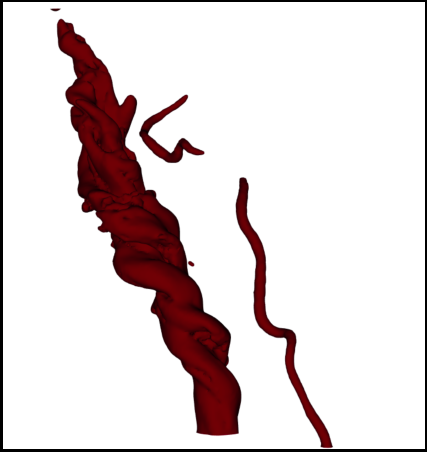
\includegraphics[width=0.9\linewidth]{Images/Tornado/zls.pdf}
\vspace{-1mm}
\caption{$ZLS_{T}$}
\label{fig:tornado_zls}
\end{subfigure}
\begin{subfigure}{0.20\linewidth}
\centering
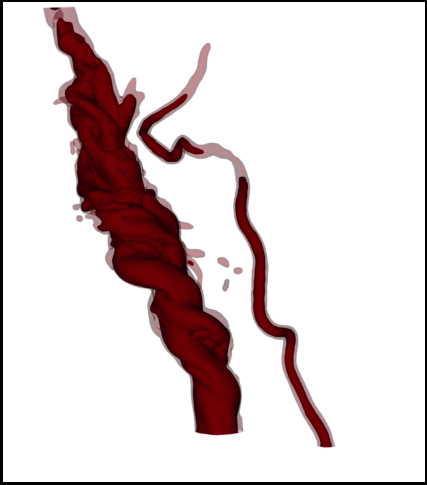
\includegraphics[width=0.9\linewidth]{Images/Tornado/fcls_50.pdf}
\vspace{-1mm}
\caption{+ $FCLS_{T,50\%}$}
\label{fig:tornado_fls}
\end{subfigure}
\begin{subfigure}{0.20\linewidth}
\centering
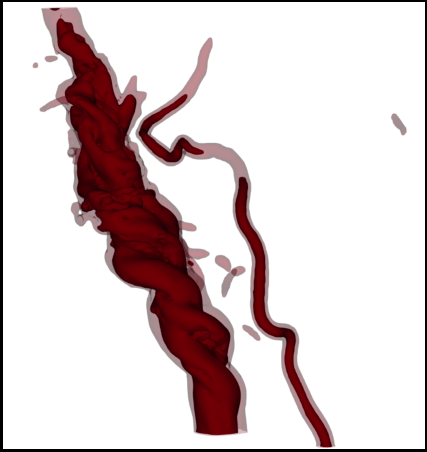
\includegraphics[width=0.9\linewidth]{Images/Tornado/fcls_68.pdf}
\vspace{-1mm}
\caption{+ $FCLS_{T,68\%}$}
\label{fig:tornado_fls}
\end{subfigure}
\begin{subfigure}{0.20\linewidth}
\centering
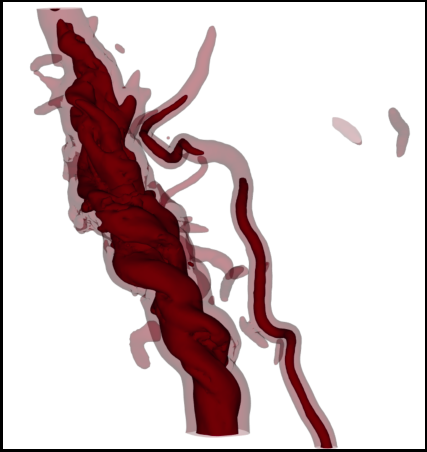
\includegraphics[width=0.9\linewidth]{Images/Tornado/fcls_95.pdf}
\vspace{-1mm}
\caption{+ $FCLS_{T,95\%}$}
\label{fig:tornado_fcls}
\end{subfigure}
\hfill
\begin{subfigure}{0.17\linewidth}
\centering
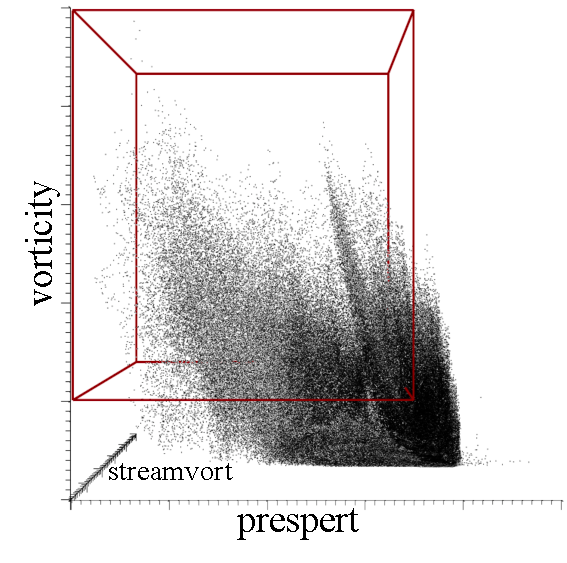
\includegraphics[width=\linewidth]{Images/Tornado/scatterplot3d.pdf}
\vspace{-4mm}
\caption{3D scatterplot of $\mathcal{A}$ and $T$ (red cuboid).} 
\label{fig:tornado_scatterplot}
\end{subfigure}
%\vspace{-2mm}
\caption{Visualization of EF-5 tornado vortices using vorticity, prespert and streamvort attributes. As in Figure~\ref{fig:tangle}, $FCLS_{T,C}$ formed wider envelopes as $C$ increased. Importantly, $FCLS_{T,C}$ visualized vortical structures of interest in the vicinity of the primary tornado vortex.}
%\vspace{-1mm}
\label{fig:tornado}
\end{figure*}

\begin{figure*}[h]
\begin{subfigure}{0.18\linewidth}
\centering
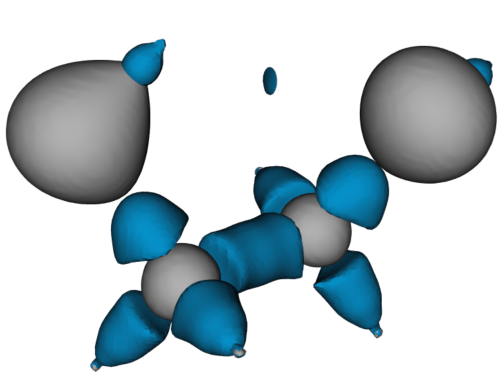
\includegraphics[width=\linewidth]{Images/EthaneDiol/gt.pdf}
\caption{$Rho_{isoval}=1.57$ (gray),\\ $s_{isoval}=-0.575$ (light blue)}
\label{}
\end{subfigure}
\begin{subfigure}{0.18\linewidth}
\centering
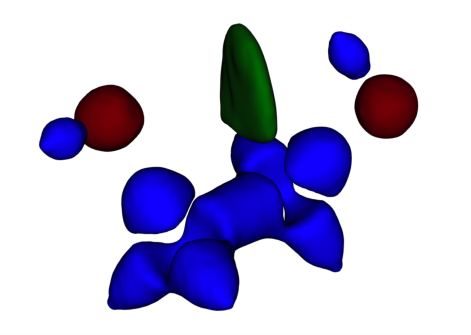
\includegraphics[width=\linewidth]{Images/EthaneDiol/zls_3.pdf}
\caption{$ZLS_{T}$}
\label{}
\end{subfigure}
\begin{subfigure}{0.18\linewidth}
\centering
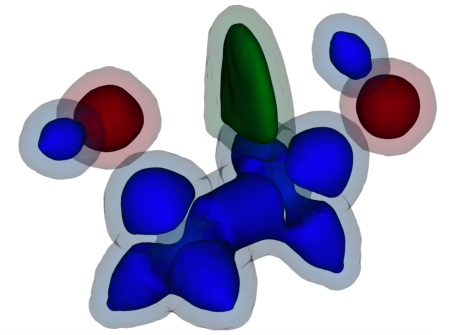
\includegraphics[width=\linewidth]{Images/EthaneDiol/fls_2_3.pdf}
\caption{$ZLS_{T}$ + $FLS_{T,2}$}
\label{}
\end{subfigure}
\begin{subfigure}{0.18\linewidth}
\centering
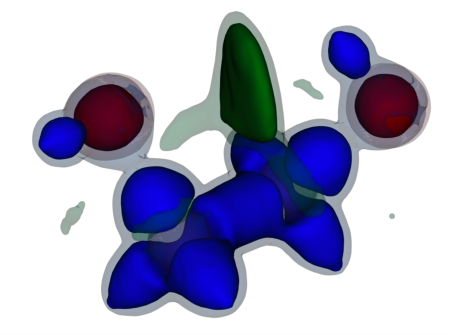
\includegraphics[width=\linewidth]{Images/EthaneDiol/fcls_68_3.pdf}
\caption{$ZLS_{T}$ + $FCLS_{T,68\%}$}
\label{}
\end{subfigure}
\begin{subfigure}{0.24\linewidth}
\centering
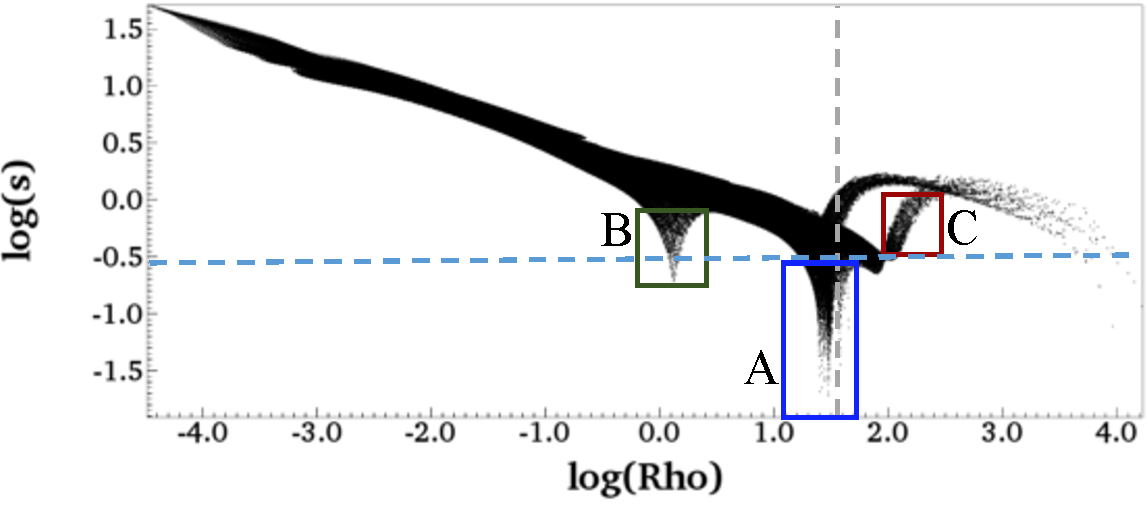
\includegraphics[width=\linewidth]{Images/EthaneDiol/scatterplot_3.pdf}
\caption{Attribute space 2D scatterplot, traits (labeled rectangular selections), and isovalues (dashed lines). We use $T = \left\{T_{A}, T_{B}, T_{C}\right\}$.} 
\label{}
\end{subfigure}
\caption{}
\label{}
\end{figure*}

\begin{figure*}[!h]
\begin{subfigure}{0.245\linewidth}
\centering
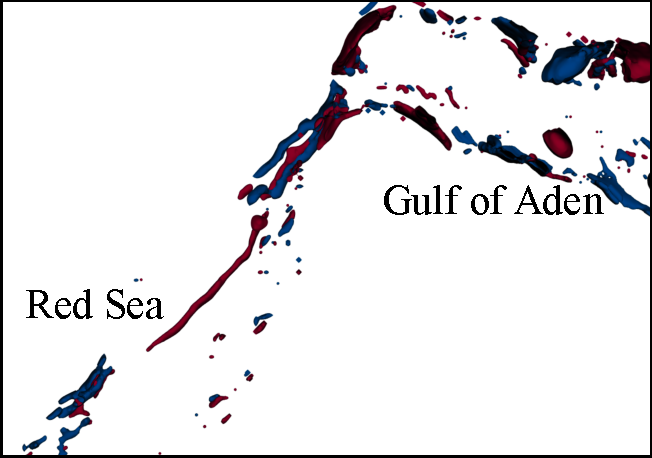
\includegraphics[width=\linewidth]{Images/RedSeaEddy/zls.pdf}
\vspace{-2mm}
\caption{$ZLS_{T}$}
\label{fig:rse_zls}
\end{subfigure}
\begin{subfigure}{0.245\linewidth}
\centering
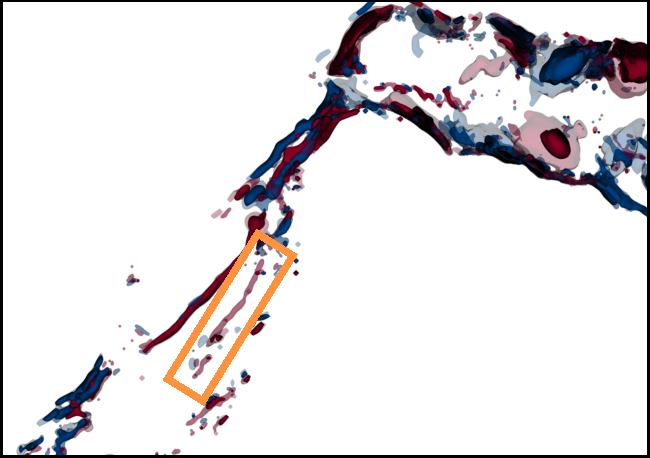
\includegraphics[width=\linewidth]{Images/RedSeaEddy/fcls_50.pdf}
\vspace{-2mm}
\caption{$ZLS_{T}$ + $FCLS_{T,50\%}$}
\label{fig:rse_fls}
\end{subfigure}
\begin{subfigure}{0.245\linewidth}
\centering
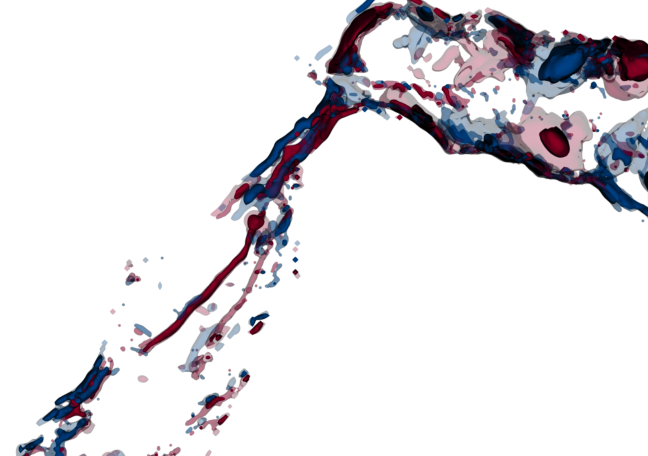
\includegraphics[width=\linewidth]{Images/RedSeaEddy/fcls_68.pdf}
\vspace{-2mm}
\caption{$ZLS_{T}$ + $FCLS_{T,68\%}$}
\label{fig:rse_fcls}
\end{subfigure}
\hfill
\begin{subfigure}{0.24\linewidth}
\centering
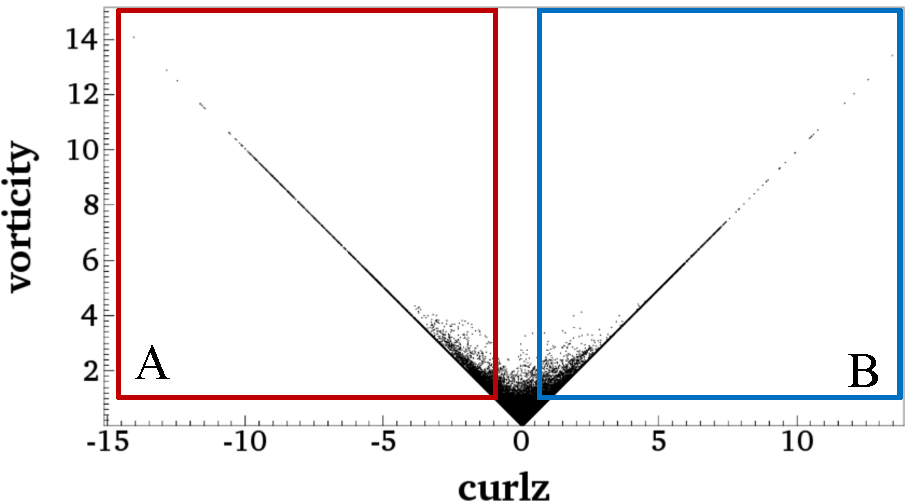
\includegraphics[width=0.95\linewidth]{Images/RedSeaEddy/scatterplot.pdf}
\vspace{-2mm}
\caption{Attribute space 2D scatterplot and traits (labeled rectangular selections). We use $T = \left\{T_{A}, T_{B}\right\}$.} 
\label{fig:rse_scatterplot}
\end{subfigure}
\vspace{-2mm}
\caption{Visualization of anticyclonic~($T_{A}$, red) and cyclonic~($T_{B}$, blue) eddies in the Gulf of Aden and part of the Red Sea using the derived attributes of vorticity magnitude and the z-component of curl. For this ensemble data set, $FCLS_{T,C}$ visualized additional paths and regions with eddies. The orange box in (c) highlights one such example.}
%\vspace{-1mm}
\label{fig:rse}
\end{figure*}

\begin{figure*}[!h]
\begin{subfigure}{0.2\linewidth}
\centering
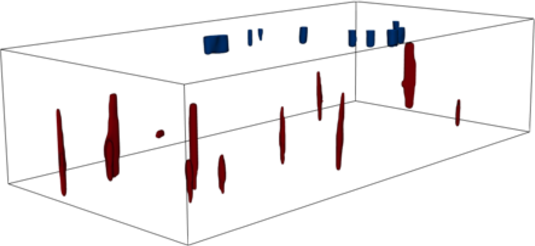
\includegraphics[width=\linewidth]{Images/Mantel/zls.pdf}
\vspace{-5mm}
\caption{$ZLS_{T}$}
\label{fig:mantel_zls}
\end{subfigure}
\begin{subfigure}{0.2\linewidth}
\centering
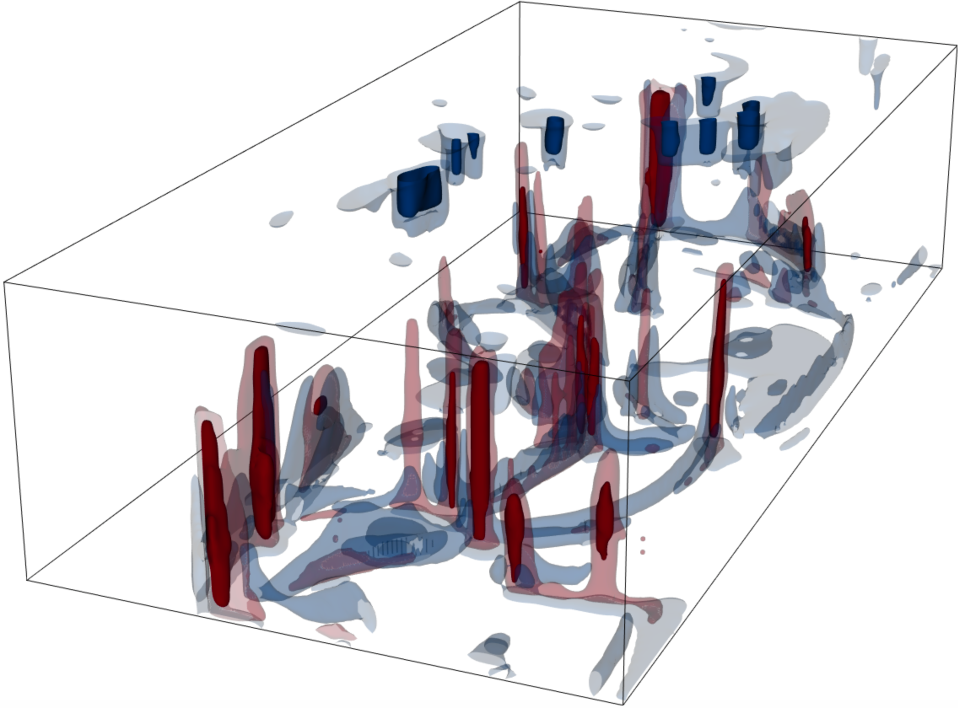
\includegraphics[width=\linewidth]{Images/Mantel/fcls_68.pdf}
\vspace{-5mm}
\caption{$ZLS_{T}$ + $FCLS_{T,68\%}$}
\label{fig:mantel_fls}
\end{subfigure}
\begin{subfigure}{0.295\linewidth}
\centering
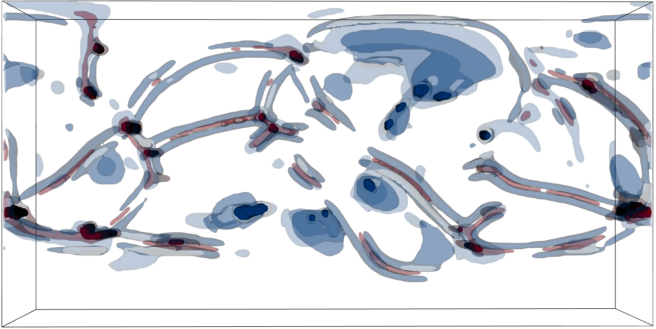
\includegraphics[width=0.9\linewidth]{Images/Mantel/fcls_68_v2.pdf}
\caption{$ZLS_{T}$ + $FCLS_{T,68\%}$}
\label{fig:mantel_fcls}
\end{subfigure}
\hfill
\begin{subfigure}{0.295\linewidth}
\centering
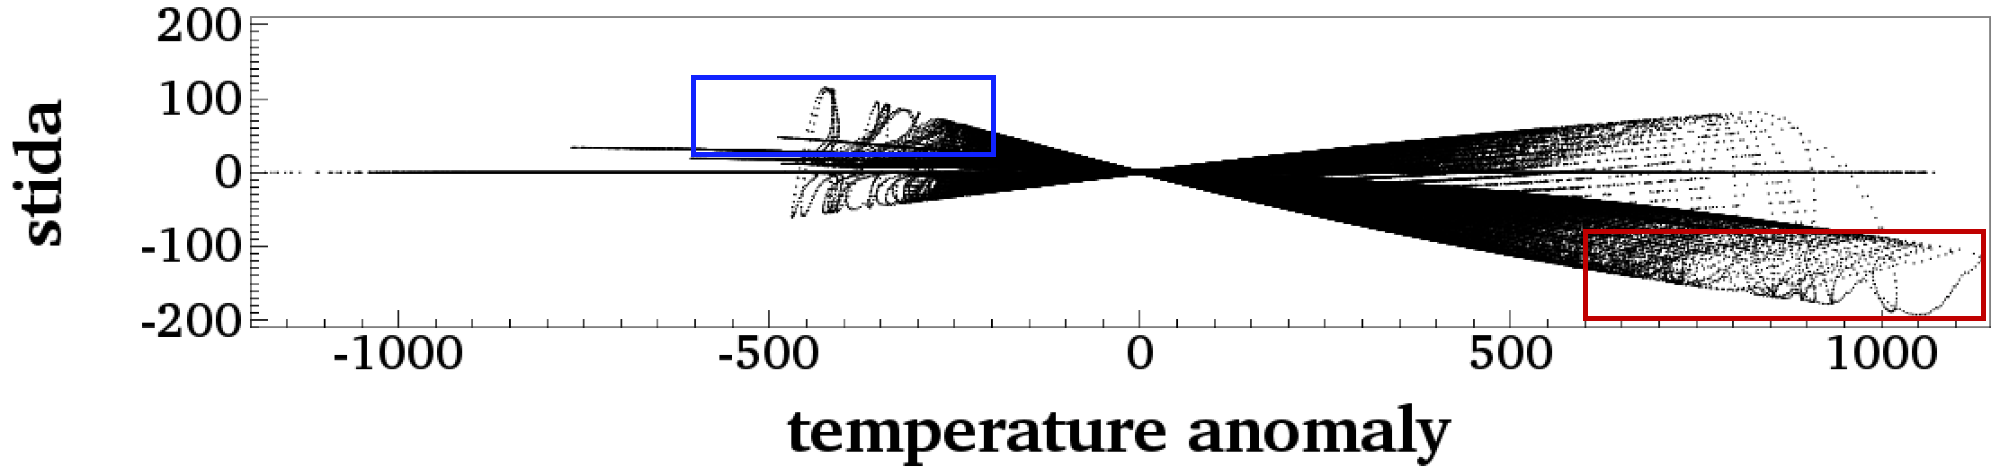
\includegraphics[width=\linewidth]{Images/Mantel/scatterplot.pdf}
%\vspace{-2mm}
\caption{Attribute space 2D scatterplot and traits (labeled rectangular selections). We use $T = \left\{T_{A}, T_{B}\right\}$.} 
\label{fig:mantel_scatterplot}
\end{subfigure}
\vspace{-2mm}
\caption{Visualization of rising hot plumes~($T_{A}$, red) and sinking material~($T_{B}$, blue) flow patterns in a subset of the spatial domain for the mantel data using the temperature anomaly and spin transition induced density anomaly~(stida) attributes.}
\label{fig:mantel}
\end{figure*}

%\begin{figure*}[!h]
\begin{subfigure}{0.195\linewidth}
\centering
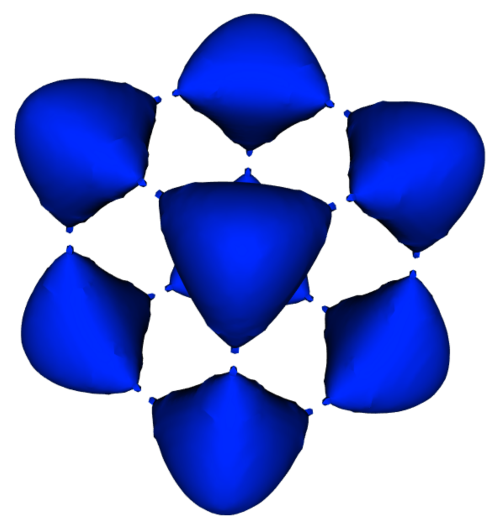
\includegraphics[width=0.8\linewidth]{Images/Tangle/gt.pdf}
\vspace{-2mm}
\caption{Ground truth, $isoval=62$}
\label{fig:tangle_gt}
\end{subfigure}
\begin{subfigure}{0.195\linewidth}
\centering
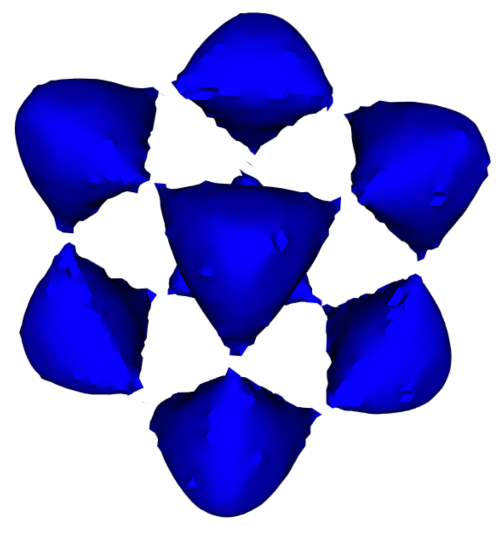
\includegraphics[width=0.8\linewidth]{Images/Tangle/zls.pdf}
\vspace{-2mm}
\caption{$ZLS_{T}$}
\label{fig:tangle_zls}
\end{subfigure}
\begin{subfigure}{0.195\linewidth}
\centering
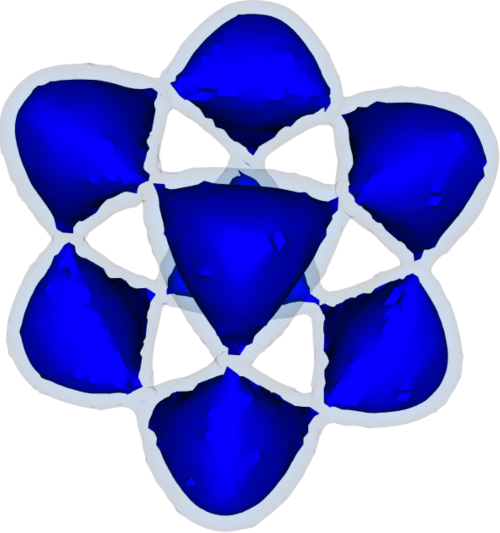
\includegraphics[width=0.8\linewidth]{Images/Tangle/fls.pdf}
\vspace{-2mm}
\caption{$ZLS_{T}$ + $FLS_{T,2}$}
\label{fig:tangle_fls}
\end{subfigure}
\begin{subfigure}{0.195\linewidth}
\centering
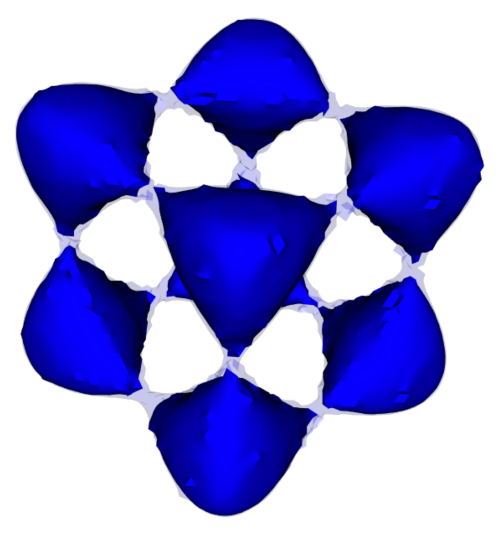
\includegraphics[width=0.8\linewidth]{Images/Tangle/fcls_68.pdf}
\vspace{-2mm}
\caption{$ZLS_{T}$ + $FCLS_{T,68\%}$}
\label{fig:tangle_fcls_68}
\end{subfigure}
\begin{subfigure}{0.195\linewidth}
\centering
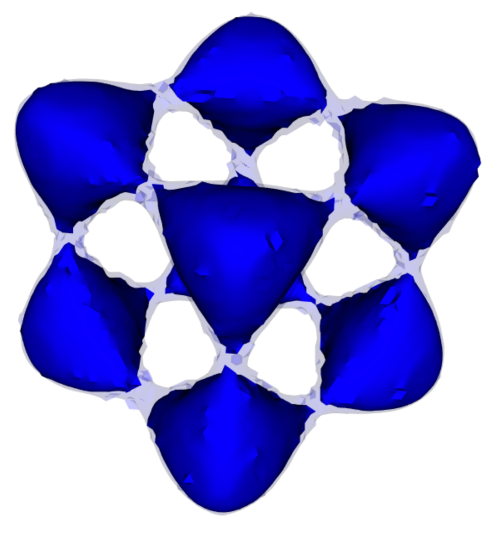
\includegraphics[width=0.8\linewidth]{Images/Tangle/fcls_95.pdf}
\vspace{-2mm}
\caption{$ZLS_{T}$ + $FCLS_{T,95\%}$}
\label{fig:tangle_fcls_95}
\end{subfigure}
\vspace{-2mm}
\caption{Visualization of sensitivity of the tangle function near values that form links between the multiple blobs. We use $T=[0,62]$.}
\vspace{-2mm}
\label{fig:tangle}
\end{figure*}

We demonstrated the use of feature confidence level-sets using five data sets.
%
Specifically, we considered an analytical tangle function~\cite{knoll2009fast}, an EF-5 Tornado~\cite{atmos10100578}, an ethanediol molecule from a chemistry simulation, Red Sea and Gulf of Aden~(RSGOA) eddy ensemble~\cite{sanikommu2020impact} and Earth's mantel convection~\cite{shahnas2017mid} data.
%
We defined between one to three traits per data set based on features of interest. 
%
%While our study demonstrated feature confidence level-sets for univariate and bivariate data, the approach can be applied to higher dimensions.\fix{Can we get an example in for a third?***}
%\fix{(Should we remove the part "the approach can be applied to higher dimensions" since we do not have results for n>2, but we can state the same in the future work section?)}.
%
In this study, each attribute was represented using a $mean$ and $SD$ field. 
%
For the RSGOA data set, we computed $mean$ and $SD$ fields from using 20 ensemble members. 
%
For other data sets, we synthetically estimated $SD$ for each scalar field of the multivariate data at each grid point by sampling the local neighborhood.
%
To evaluate our technique, we visualized the $ZLS_{T}$ both in isolation and augmented with $FCLS_{T,C}$. 
%
When visualized together, the $ZLS_{T}$ is shown using an opaque isosurface, and the $FCLS_{T,C}$ is shown using an isosurface colored with the same hue and 25\% opacity.
%
We used VisIt~\cite{childs2012visit} in our pipeline to render level-sets.

%also augment it with a semi-opaque, single feature level-set $FLS_{T,K}$ for some level $K$, or a feature confidence level-set $FCLS_{T,C}$ for some confidence $C$ (and level $\epsilon$).
%

%For all data sets considered, as expected we found $FLS_{T,K}$ has the shortcoming of discernibility.
%
%The $FLS_{T,K}$ level-set typically formed a ``shell'' like structure.
%
Across all data sets, the shape of $FCLS_{T,C}$ corresponded to the uncertainty of the data in the spatial domain.
%
For example, for the analytical tangle function where uncertainty is higher near the links between the blobs for the trait specified, we found comparing Figures~\ref{fig:tangle_fcls_68} and~\ref{fig:tangle_fcls_95} the $FCLS_{T,C}$ envelope expanded between the links in response to increasing the value of $C$, but not significantly on the exterior of the blob surface.
%
By leveraging the information pertaining to field distribution~($mean$, $SD$), $FCLS_{T,C}$ provided secondary structure visualization based on uncertainty.
%
%\fix{(Should we add boxes/zoomed-in views to the examples below to illustrate improvements achieved using our  $FCLS_{T,C}$? For example, we may show boxes where molecular topology is discovered nicely or one link and one blob in the case of the tangle function. This will enhance the interpretability of results.)}
%
For example, we observed the structure of weaker tornado vortices~(Figure~\ref{fig:tornado}), topological structure information for the ethanediol molecule~(Figure~\ref{fig:ethanediol}), regions with anticyclonic and cyclonic eddies across ensemble members~(Figure~\ref{fig:rse}), and the proximity as well as relationship of contrasting features in the spatial domain for the mantel data set~(Figure~\ref{fig:mantel_fcls_68_v2}).
%
%Importantly, for the traits selected, the secondary structures produced using $FCLS_{T,C}$ did not overlap one another.
%
%In contrast, for the same traits, $FLS_{T,K}$ resulted in overlapping and occluding level-sets~(see Figure~\ref{fig:rse_fls}).
%
%We provide supplementary visualizations and comparisons in the additional material. 
 


\section{Future Work and Conclusion}
\label{sec:conclusion}
In this paper, we proposed feature confidence level-sets and demonstrated their use for uncertain multivariate data sets.
%
There remain, however, several opportunities for future work in this direction.
%
These include evaluations of feature confidence level-sets on
parametric and non-parametric density models, application of attribute-specific confidence interval percentages, 
visualization of derived feature probability fields, and visualizations of mappings of uncertain multivariate data between the spatial domain and attribute space.
%
Further, although we considered a simplified trait definition, intuitive trait specification interfaces 
that include controls to specify confidence for higher dimensional data remain an open research challenge. 

Overall, we contributed a technique to visualize uncertain multivariate data via feature level-sets.
%
Our study demonstrated the ability of the approach to visualize regions of uncertainty in relation to a specific trait or feature and the improved secondary feature structure visualization that feature confidence level-sets offer.

